\documentclass[tikz]{standalone}
\usetikzlibrary{calc,intersections}
\begin{document}
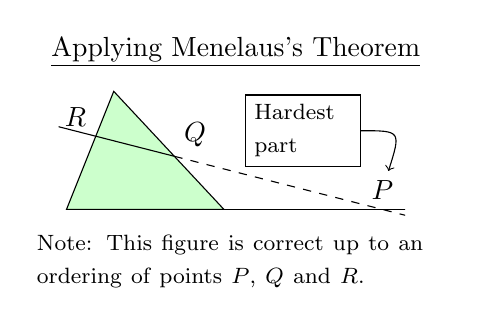
\begin{tikzpicture}
  \coordinate (A) at (0,0);
  \coordinate (B) at (2,0);
  \coordinate (C) at (0.6,1.5);
  \path[draw,fill=green!20] (A) -- (B) -- (C) -- cycle;
  % Title
  \node [align=center] at (2.15,2.0)
    {\underline{Applying Menelaus's Theorem}};
  % Remarks
  \node [anchor=north west,text width=150] at (-.5,-.2)
    {\footnotesize Note: This figure is correct up to an ordering of
     points $P$, $Q$ and $R$.};
  \clip (-.1,-.1) rectangle (4.3,1.6);
  %\draw [help lines, step=.5] (0,0) grid (5,2); %Help lines
  \coordinate [label=above right:$Q$] (Q) at ($ (B) ! .45 ! (C) $);
  \coordinate [label=above left:$R$] (R) at ($ (C) ! .38 ! (A) $);
  \draw ($ (R) ! -1 ! (Q) $) -- (R) -- (Q);
  \draw [name path=ExtLine,dashed] (Q) -- ($ (R) ! 5 ! (Q) $);
  \draw [name path=Side] (B) -- ($ (A) ! 2.5 ! (B) $);
  \path [name intersections={of=ExtLine and Side, by={[label={[name=lblP]above:$P$}]P}}];
  \node [draw,text width=35] (box) at (3,1)
    {\footnotesize Hardest part};
  \draw [->] (box.east) .. controls (4.25,1) .. (lblP);
\end{tikzpicture}
\end{document}
